\section{时间可测的方程}
\label{sec:odeex-measurable}

前面的结论都要求右端对时间连续，但外部输入经常不连续。电路开关闭合、暖气切换功率时，输入在某些时刻跳变；更一般的输入可能只是一个可积函数。第~\ref{chap:ordinary-differential-equations}章已经看到，这类方程的解在跳变处有折角，不处处可微，要用积分方程来确定。对这样的右端，解的存在、唯一和延拓分别需要什么条件？

\paragraph{一个切换输入}
取$\dot x=-x+g(t)$，$x(0)=0$，其中$g(t)=1$（$0\leq t<1$），$g(t)=0$（$t\geq1$）。在$[0,1]$上解得
\[
 x(t)=1-\mathrm{e}^{-t},
\]
到$t=1$时$x(1)=1-\mathrm{e}^{-1}\approx0.632$。之后从这个值开始按齐次方程衰减，
\[
 x(t)=(1-\mathrm{e}^{-1})\,\mathrm{e}^{-(t-1)},\qquad t\geq1.
\]

两段在$t=1$处连续，但左导数是$\mathrm{e}^{-1}\approx0.368$，右导数是$-(1-\mathrm{e}^{-1})\approx-0.632$，如图~\ref{fig:odeex-measurable-switch}(b)。曲线处处满足积分方程，只在$t=1$这一点没有导数。

输入还可以无界。图~\ref{fig:odeex-measurable-switch}(c)的$\dot x=t^{-1/2}$，$x(0)=0$，在$t=0$处右端没有有限值，积分却收敛，解是$x=2\sqrt{t}$，在起点的切线是竖直的。把输入换成$1/t$就不行了：$\int_0^t\mathrm{d}s/s$发散，从$x(0)=0$出发的解不存在。可见起作用的不是有界性，而是右端在时间上可积。

\begin{BookInlineFigure}
  \centering
  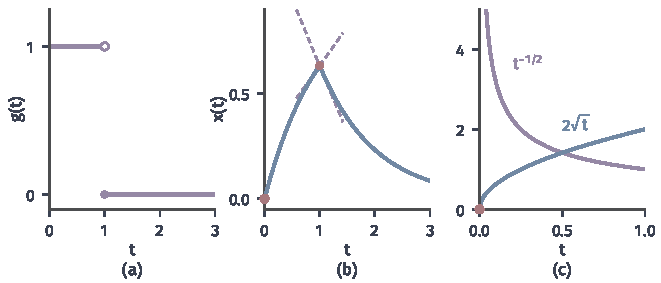
\includegraphics[width=112mm]{figures/06-differential-equations/01-ordinary-differential-equations/matplotlib/odeex-measurable-switch/figure.pdf}
  \caption{时间可测的右端。(a)切换输入$g$（紫线）。(b)$\dot x=-x+g(t)$，$x(0)=0$的解（蓝线），在$t=1$有折角，紫色虚线是左右两侧的切线。(c)无界但可积的输入$t^{-1/2}$（紫线）和解$2\sqrt{t}$（蓝线）。}
  \label{fig:odeex-measurable-switch}
\end{BookInlineFigure}

\paragraph{条件与解的定义}
把上面的观察写成条件。下面$J$是区间，$\bm{\Omega}\subseteq\mathbb{R}^{n}$是开集。

\begin{definition}[Carathéodory条件]
\label{def:odeex-caratheodory}
称$\bm{f}:J\times\bm{\Omega}\to\mathbb{R}^{n}$满足\term{Carathéodory条件}（Carathéodory conditions），是指：
\begin{enumerate}
 \item 对每个$\bm{x}\in\bm{\Omega}$，$t\mapsto\bm{f}(t,\bm{x})$是Lebesgue可测的；
 \item 对几乎每个$t\in J$，$\bm{x}\mapsto\bm{f}(t,\bm{x})$连续；
 \item 对每个紧区间$J'\subseteq J$和紧集$\bm{C}\subseteq\bm{\Omega}$，存在$m\in L^1(J')$，使对几乎每个$t\in J'$和所有$\bm{x}\in\bm{C}$，都有
 \begin{equation}
 \lVert\bm{f}(t,\bm{x})\rVert_2\leq m(t).
 \label{eq:odeex-caratheodory-bound}
 \end{equation}
\end{enumerate}
\end{definition}

第三条是局部可积的上界，它取代了连续函数在紧集上有界这件事。解的概念也要放宽。若$I\subseteq J$是含$t_0$的区间，$\bm{x}:I\to\bm{\Omega}$在每个紧子区间上绝对连续，$\bm{x}(t_0)=\bm{x}_0$，并且对几乎每个$t\in I$有$\dot{\bm{x}}(t)=\bm{f}(t,\bm{x}(t))$，就称$\bm{x}$是\term{Carathéodory解}（Carathéodory solution）。

绝对连续恰好使“几乎处处的导数”能积分回函数本身。因此这样的解就是满足积分方程~\eqref{eq:odeex-integral}的连续曲线，积分取Lebesgue意义。

绝对连续这一要求不能换成“连续且几乎处处满足方程”。图~\ref{fig:odeex-cantor-false}中的Cantor函数$c$在$[0,1]$上连续，几乎处处导数为零，并且$c(0)=0$。如果只看几乎处处的导数，$c$就满足$\dot x=0$，$x(0)=0$，唯一性立刻失败；但$c(1)=1$，积分方程的右端却恒为$0$，它不是Carathéodory解。

\begin{BookInlineFigure}
  \centering
  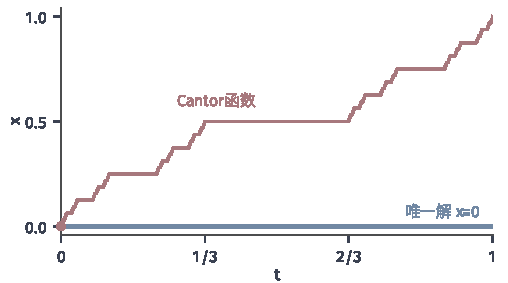
\includegraphics[width=86mm]{figures/06-differential-equations/01-ordinary-differential-equations/matplotlib/odeex-cantor-false/figure.pdf}
  \caption{绝对连续的必要性。方程是$\dot x=0$，$x(0)=0$，蓝线是它的唯一解$x\equiv0$。红线是Cantor函数，连续并几乎处处导数为零，但不绝对连续，不满足积分方程，因而不算解。}
  \label{fig:odeex-cantor-false}
\end{BookInlineFigure}

\paragraph{沿曲线的可测性}
积分方程要有意义，$s\mapsto\bm{f}(s,\bm{y}(s))$必须可测。条件只分别给出了对时间的可测性和对状态的连续性，下面的引理把两者合起来。

\begin{lemma}[沿连续曲线的可测性]
\label{lem:odeex-composition-measurable}
设$\bm{f}$满足定义~\ref{def:odeex-caratheodory}，$J'\subseteq J$是紧区间，$\bm{y}:J'\to\bm{C}$连续，$\bm{C}\subseteq\bm{\Omega}$紧。则$s\mapsto\bm{f}(s,\bm{y}(s))$在$J'$上可测，且可积。
\end{lemma}

\begin{proof}
把$J'$等分为$2^j$段，令$\bm{y}_j$在每段上取$\bm{y}$在该段左端点的值，右端点处取$\bm{y}$的值。在每段上$\bm{y}_j$是常向量，由条件1，$s\mapsto\bm{f}(s,\bm{y}_j(s))$在每段上可测，从而在$J'$上可测。

$\bm{y}$连续，所以$\bm{y}_j(s)\to\bm{y}(s)$对每个$s$成立。由条件2，对几乎每个$s$，$\bm{f}(s,\bm{y}_j(s))\to\bm{f}(s,\bm{y}(s))$。可测函数列的几乎处处极限可测，所以$\bm{f}(s,\bm{y}(s))$可测。可积性由式~\eqref{eq:odeex-caratheodory-bound}得到。
\end{proof}

\paragraph{局部存在}
Euler折线在这里不能用了。Euler格式需要右端在网格时刻$t_k$的值，而可测函数在单点的值没有意义，改变零测集上的值不改变方程，却能任意改变Euler格式。

替代办法是Tonelli的延迟逼近：用稍早一段的已知曲线计算积分，这样积分号里永远只含已经算好的部分，不需要逐点取值。

\begin{theorem}[Carathéodory存在定理]
\label{thm:odeex-caratheodory-existence}
设$\bm{f}$满足定义~\ref{def:odeex-caratheodory}，$[t_0,t_0+a]\subseteq J$，$\bm{B}_b\subseteq\bm{\Omega}$，$m\in L^1([t_0,t_0+a])$是$\bm{C}=\bm{B}_b$上的式~\eqref{eq:odeex-caratheodory-bound}的上界。取$\delta\in(0,a]$，使
\begin{equation}
 \int_{t_0}^{t_0+\delta}m(s)\,\mathrm{d}s\leq b.
 \label{eq:odeex-caratheodory-window}
\end{equation}
则初值问题在$[t_0,t_0+\delta]$上有取值于$\bm{B}_b$的Carathéodory解。$t_0$左侧有对称的结论。
\end{theorem}

积分$\int_{t_0}^{t_0+\delta}m$在$\delta\to0$时趋于零，满足式~\eqref{eq:odeex-caratheodory-window}的$\delta$总存在。它是$\delta\leq b/M$的自然推广：盒子的高度$b$现在由累计的速度上限来消耗。

\begin{proof}
\emph{延迟逼近。}记$I^+=[t_0,t_0+\delta]$，对正整数$N$，记$r=\delta/N$。定义$\bm{y}_N$：在$[t_0,t_0+r]$上$\bm{y}_N\equiv\bm{x}_0$；对$t\in(t_0+r,t_0+\delta]$，
\[
 \bm{y}_N(t)=\bm{x}_0+\int_{t_0}^{t-r}\bm{f}(s,\bm{y}_N(s))\,\mathrm{d}s.
\]
这个定义逐段进行：$t$在第$j+1$段时，积分只用到前$j$段上已定义的$\bm{y}_N$。由引理~\ref{lem:odeex-composition-measurable}，积分有定义。由式~\eqref{eq:odeex-caratheodory-window}，
\[
 \lVert\bm{y}_N(t)-\bm{x}_0\rVert_2\leq\int_{t_0}^{t-r}m(s)\,\mathrm{d}s\leq b,
\]
所以$\bm{y}_N$的取值都在$\bm{B}_b$中，递推能够继续。

\emph{等度连续。}令$W(\rho)$为$m$在$I^+$中长度不超过$\rho$的区间上积分的最大值。Lebesgue积分的绝对连续性给出$\rho\to0$时$W(\rho)\to0$。对$s<t$，$\bm{y}_N(t)-\bm{y}_N(s)$是一段长度不超过$t-s$的区间上的积分（或为零），所以
\[
 \lVert\bm{y}_N(t)-\bm{y}_N(s)\rVert_2\leq W(t-s).
\]
界$W$对所有$N$相同，$\{\bm{y}_N\}$一致有界且等度连续。由Arzelà--Ascoli判据，存在子列在$I^+$上一致收敛到连续曲线$\bm{x}:I^+\to\bm{B}_b$。

\emph{取极限。}把延迟积分写成到$t$的积分减去尾部，对所有$t\in I^+$（$t<t_0+r$时也成立）有
\[
 \bm{y}_N(t)=\bm{x}_0+\int_{t_0}^{t}\bm{f}(s,\bm{y}_N(s))\,\mathrm{d}s-\bm{E}_N(t),\qquad
 \lVert\bm{E}_N(t)\rVert_2\leq W(r).
\]
沿子列，$\bm{y}_N(s)\to\bm{x}(s)$，由条件2，对几乎每个$s$，$\bm{f}(s,\bm{y}_N(s))\to\bm{f}(s,\bm{x}(s))$。被积函数以$m$为可积控制，由控制收敛定理，积分收敛。尾部$\bm{E}_N$趋于零。

令$N\to\infty$，$\bm{x}$满足积分方程~\eqref{eq:odeex-integral}，因而是Carathéodory解。左侧用时间反演$s\mapsto2t_0-s$得到。
\end{proof}

图~\ref{fig:odeex-tonelli-delay}对切换输入的例子画出了延迟逼近。开头的一段$r$内曲线不动，因为积分尚未开始；之后曲线滞后真解一段时间，$N$增大时滞后变短，逐渐贴合真解。

\begin{BookInlineFigure}
  \centering
  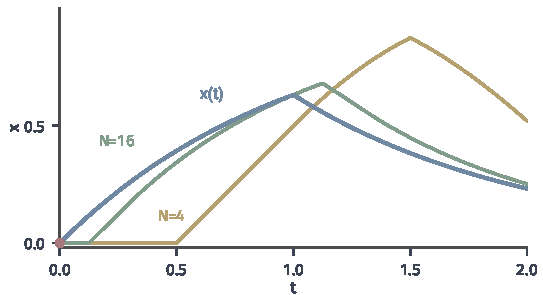
\includegraphics[width=92mm]{figures/06-differential-equations/01-ordinary-differential-equations/matplotlib/odeex-tonelli-delay/figure.pdf}
  \caption{延迟逼近。方程是$\dot x=-x+g(t)$，$x(0)=0$，$g$是图~\ref{fig:odeex-measurable-switch}(a)的切换输入，$\delta=2$。蓝线是解，黄线和绿线是$N=4$和$N=16$的延迟逼近$y_N$，延迟长度$r=\delta/N$。}
  \label{fig:odeex-tonelli-delay}
\end{BookInlineFigure}

\paragraph{唯一性}
存在定理对状态只要求连续，唯一性仍要另外的条件。第~\ref{sec:odeex-uniqueness}节的最后一个反例说明，对时间不一致的Lipschitz常数可以破坏唯一性；但$L$不必有界，可以放宽到$L$随时间局部可积。

\begin{theorem}[可积Lipschitz系数下的唯一性]
\label{thm:odeex-caratheodory-unique}
在定理~\ref{thm:odeex-caratheodory-existence}的记号下，设存在$\ell\in L^1([t_0,t_0+a])$，使对几乎每个$t\in[t_0,t_0+a]$和所有$\bm{x},\bm{y}\in\bm{B}_b$，
\begin{equation}
 \lVert\bm{f}(t,\bm{x})-\bm{f}(t,\bm{y})\rVert_2\leq\ell(t)\lVert\bm{x}-\bm{y}\rVert_2.
 \label{eq:odeex-integrable-lipschitz}
\end{equation}
取$\delta\in(0,a]$满足式~\eqref{eq:odeex-caratheodory-window}，以及
\begin{equation}
 \int_{t_0}^{t_0+\delta}\ell(s)\,\mathrm{d}s\leq\frac12.
 \label{eq:odeex-integrable-window}
\end{equation}
则初值问题在$[t_0,t_0+\delta]$上恰有一个取值于$\bm{B}_b$的Carathéodory解，Picard迭代~\eqref{eq:odeex-picard-iteration}一致收敛到它，并满足式~\eqref{eq:odeex-picard-error}。
\end{theorem}

\begin{proof}
证明与定理~\ref{thm:odeex-picard-lindelof}逐步对应。令$\mathcal{X}$为$[t_0,t_0+\delta]$上取值于$\bm{B}_b$的连续曲线组成的集合，它在一致距离下完备。

对$\bm{u}\in\mathcal{X}$，由引理~\ref{lem:odeex-composition-measurable}，$\mathcal{T}\bm{u}$有定义且连续，由式~\eqref{eq:odeex-caratheodory-window}，其取值在$\bm{B}_b$中。对$\bm{u},\bm{v}\in\mathcal{X}$，由式~\eqref{eq:odeex-integrable-lipschitz}和式~\eqref{eq:odeex-integrable-window}，
\[
 \lVert\mathcal{T}\bm{u}-\mathcal{T}\bm{v}\rVert_{\infty}
 \leq\int_{t_0}^{t_0+\delta}\ell(s)\lVert\bm{u}(s)-\bm{v}(s)\rVert_2\,\mathrm{d}s
 \leq\frac12\lVert\bm{u}-\bm{v}\rVert_{\infty}.
\]
由压缩映射定理得到唯一的不动点，它满足积分方程。取值于$\bm{B}_b$的Carathéodory解都是$\mathcal{T}$的不动点，所以都等于它。
\end{proof}

这里的压缩常数不再是“$L$乘时间”，而是系数的累计量$\int\ell$，后者由积分的绝对连续性保证在短时间内很小。一个解若从$\bm{x}_0$出发，由连续性在一小段时间内留在$\bm{B}_b$中，所以两条解在初始时刻重合后，局部总是相同的。

\begin{example}[系数无界的唯一性]
\label{ex:odeex-integrable-lipschitz}
考虑$\dot x=x/(2\sqrt{t})$，$x(0)=1$，取$b=1$。在$\lvert x-1\rvert\leq1$上，上界和Lipschitz系数分别可取
\[
 m(t)=\frac{1}{\sqrt{t}},\qquad\ell(t)=\frac{1}{2\sqrt{t}}.
\]
两者在$t\to0$时无界，但都可积。由$\int_0^\delta m=2\sqrt{\delta}$和$\int_0^\delta\ell=\sqrt{\delta}$，取$\delta=1/4$，式~\eqref{eq:odeex-caratheodory-window}和式~\eqref{eq:odeex-integrable-window}都成立。

从$x^{(0)}=1$出发迭代，第一步对$1/(2\sqrt{s})$积分，第二步对$(1+\sqrt{s})/(2\sqrt{s})$积分，分别得到
\[
 x^{(1)}=1+\sqrt{t},\qquad x^{(2)}=1+\sqrt{t}+\frac{t}{2}.
\]

一般地，$x^{(k)}=\sum_{j=0}^{k}(\sqrt{t})^j/j!$，极限是$\mathrm{e}^{\sqrt{t}}$。在$t=1/4$处，三轮迭代的取值依次是
\[
 1.5,\quad1.625,\quad1.6458,
\]
真解是$\mathrm{e}^{1/2}\approx1.6487$。
\end{example}

图~\ref{fig:odeex-integrable-lipschitz}比较了这个例子的系数与方程~\eqref{eq:odeex-clip}的系数。$1/(2\sqrt{t})$虽然也在原点无界，但其下的面积有限，短时间窗内的累计量可以小于$1/2$；$2/t$在原点附近的面积发散，没有任何时间窗能让累计量变小，多解正是从这里产生的。

\begin{BookInlineFigure}
  \centering
  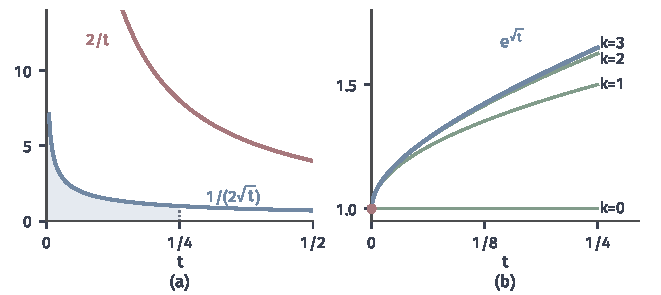
\includegraphics[width=112mm]{figures/06-differential-equations/01-ordinary-differential-equations/matplotlib/odeex-integrable-lipschitz/figure.pdf}
  \caption{时间上的Lipschitz系数。(a)蓝线$1/(2\sqrt{t})$可积，浅蓝面积是$[0,1/4]$上的累计量$1/2$；红线$2/t$在原点不可积。(b)$\dot x=x/(2\sqrt{t})$，$x(0)=1$的Picard迭代$x^{(0)},\ldots,x^{(3)}$（绿线）和解$\mathrm{e}^{\sqrt{t}}$（蓝线）。}
  \label{fig:odeex-integrable-lipschitz}
\end{BookInlineFigure}

\paragraph{唯一性不来自可测性或增长控制}
方程~\eqref{eq:odeex-sqrt}的右端满足Carathéodory条件，局部有界，并且至多线性增长，定理~\ref{thm:odeex-caratheodory-existence}保证它有解，但它有无穷多个解。时间可测性是对时间方向的放宽，增长控制处理的是解走多远，两者都不涉及两条解在状态方向上是否分开。方程~\eqref{eq:odeex-clip}也满足Carathéodory条件，它失败的原因是系数$2/t$不局部可积。

\paragraph{延拓与全局存在}
第~\ref{sec:odeex-maximal}节和第~\ref{sec:odeex-global}节的论证只用到积分方程，以及局部定理的时间窗在紧集上有统一下限，因此在下述条件下可以照搬：$\bm{f}$满足定义~\ref{def:odeex-caratheodory}，并且对每个紧区间$J'\subseteq J$和紧集$\bm{C}\subseteq\bm{\Omega}$，存在$\ell\in L^1(J')$，使式~\eqref{eq:odeex-integrable-lipschitz}在$J'\times\bm{C}$上成立。

唯一改动的地方是时间窗的选取。设$J$开，$\bm{K}\subseteq J\times\bm{\Omega}$紧，按引理~\ref{lem:odeex-uniform-window}的方式把$\bm{K}$放大成紧集，其上有共同的$m,\ell$。积分的绝对连续性给出一个$\delta_{\bm{K}}>0$，使$m$和$\ell$在任何长度不超过$\delta_{\bm{K}}$的时间段上的积分分别不超过$\rho/2$和$1/2$。

于是最大绝对连续解存在且唯一，最大存在区间在$J$中相对开，有限端点处解离开每个紧集。若增长条件~\eqref{eq:odeex-linear-growth}对几乎每个$t$成立，系数$\alpha,\beta$局部可积，定理~\ref{thm:odeex-global}及其上界~\eqref{eq:odeex-global-bound}也成立，因为那里的证明本来就只用了积分方程。切换输入的线性方程就属于这种情形，其解在整个时间轴上存在。
